


\begin{frame}{Newton iteration: Workhorse of SNES}
  \begin{flushright}
    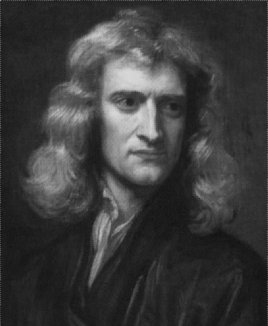
\includegraphics[width=0.25\textwidth]{figures/Newton}
  \end{flushright}
  \vspace*{-4cm}
  \begin{block}{Standard form of a nonlinear system}
    \[ \hspace*{-1cm} -\nabla \cdot \bigl(\vert\nabla u\vert^{\mathfrak{p}-2} \nabla u \bigr) - \lambda e^u = F(u) = 0 \]
  \end{block}
  
  \begin{block}{Iteration}
    \vspace*{-0.5cm}
    \begin{align*}
      \text{Solve:} & \qquad J(u) w = -F(u) \\
      \text{Update:} & \qquad u^+ \gets u + w
    \end{align*}
    \begin{itemize}
    \item Quadratically convergent near a root: $|u^{n+1}-u^*| \in \mathcal{O} \Big(|u^n-u^*|^2\Big)$
    \item Picard is the same operation with a different $J(u)$
    \end{itemize}
  \end{block}
  
  \begin{block}{Jacobian Matrix for $\mathfrak{p}$-Bratu Equation}
    \vspace*{-0.5cm}
        \begin{gather*}
         J(u) w \sim -\nabla \bigl[ (\eta {\mathbf{1}} + \eta' \nabla u \otimes \nabla u) \nabla w \bigr] - \lambda e^u w \\
          \eta' = \frac{\mathfrak{p}-2}{2} \eta / (\epsilon^2 + \gamma)
        \end{gather*}
  \end{block}
\end{frame}


